\documentclass{article}
\usepackage[a4paper, width=170mm, top=20mm, bottom=20mm]{geometry}
\usepackage{hyperref}
\usepackage{amsmath}
\usepackage{nopageno}
\usepackage{xcolor}
\usepackage{adjustbox}
\newcommand\tab[1][0.5cm]{\hspace*{#1}}
\usepackage[framemethod=default]{mdframed}
\newmdenv[linecolor=white,backgroundcolor=blue!5]{myframe}
\usepackage{graphicx}
\usepackage{subcaption}

% Set greek language
%\usepackage[english,greek]{babel}
\usepackage[utf8]{inputenc}
%\newcommand{\en}[1]{\foreignlanguage{english}{#1}}
%\usepackage{kerkis} 
%\usepackage{abc}

% Hyperref
\usepackage{hyperref}
\hypersetup{
	colorlinks=true,
	linkcolor=black,
	filecolor=black,      
	urlcolor=blue,
}

% Tables
\usepackage{tabu}
\usepackage{tabularx}
\newcolumntype{L}[1]{>{\raggedright\let\newline\\\arraybackslash\hspace{0pt}}m{#1}}
\newcolumntype{C}[1]{>{\centering\let\newline\\\arraybackslash\hspace{0pt}}m{#1}}
\newcolumntype{R}[1]{>{\raggedleft\let\newline\\\arraybackslash\hspace{0pt}}m{#1}}

\begin{document}
	

\noindent
\begin{huge}
\hspace{-3.0mm}\textbf{OpenFOAM Tutorials}
\end{huge}

%\section*{OpenFOAM Tutorials}
%\subsection*{1.0 ~ Intro}
\section{Intro}
	
\begin{enumerate}
	\item Install a Linux distribution in your computer configuration (preferably the latest \href{https://ubuntu.com/}{Ubuntu LTS} version), either alongside with Windows (dual boot) or using a Virtual Machine. The next step is to familiarize with the Linux terminal [\href{https://ubuntu.com/tutorials/command-line-for-beginners#6-a-bit-of-plumbing}{1}, \href{https://www.howtogeek.com/140679/beginner-geek-how-to-start-using-the-linux-terminal/}{2}] and the Linux OS in general.
	
	\item Successfully install the latest version of the OpenFOAM \textsuperscript{\textcopyright} open-source CFD software and the post-process tool Paraview \textsuperscript{\textcopyright} from the official website (\href{https://openfoam.org/}{https://openfoam.org/}), following the installation instructions.
	
	\item With the help of the latest version of the OpenFOAM User Guide, which can be found in the website, run the incompressible solver {\tt icoFoam} to solve the lid-driven cavity case. In order to achieve that, wither manually copy the directory with the corresponding tutorial case, which can be found in the following path (e.g. for the OpenFOAM 8 version)
	
	{\tt \tab /opt/openfoam8/tutorials/incompressible/icoFoam/cavity/cavity }
	
	into your personal OpenFOAM directory that was created in the installation process, or run the command
	
	{\tt \tab \$ cp -r \$FOAM\_TUTORIALS/incompressible/icoFoam/cavity/cavity \$FOAM\_RUN}
	
	\vspace{0.2cm}
	To solve the cavity tutorial, run the following commands:

	{\tt %
	\tab \$ cd \$FOAM\_RUN/cavity	\\%
	\tab \$ blockMesh \\%
	\tab \$ icoFoam \\%
	\tab \$ paraFoam
 	}
 
 	More information about the commands and their usage, can be found in the User Guide.
 	
 	After the successful solution of the cavity case, you can run different simulations by altering the problem's geometry, the flow parameters {\tt ./constant/transportProperties}, the boundary conditions ({\tt ./0/} directory), the solution time step $\Delta t$, the solution writing times ({\tt ./system/controlDict}), etc. Also, familiarize yourselves with the ParaView post-processing tool, and its capabilities. 
 
 	\item Modify the cavity case, from the previous step, in order to simulate the 2D laminar incompressible flow between parallel plates. It must be reminded that the maximum exit velocity must be equal to the $3/2$ of the inlet velocity.
 	
 	As for the boundary conditions, the velocity at the walls must be zero ({\tt noSlip}), {\tt uniform} (Dirichlet BC) at the inlet and {\tt zeroGradient} (Neumann BC) at the outlet of the pipe. The pressure must be {\tt zeroGradient} everywhere at the walls and inlet, except the pipe's outlet, where must be zero, as the fluid exits the pipe into the atmosphere (relative pressure). 
 	
 	The inlet and outlet boundaries type must be defined as 'patch' in the {\tt blockMeshDict} file, while all walls could be defined as either 'patch' or 'wall'. Modify the mesh in the blockMeshDict so that it is denser towards the walls, and towards the pipe’s inlet.
 	

	\begin{figure}[h]
		\begin{subfigure}{\textwidth}
			\centering
			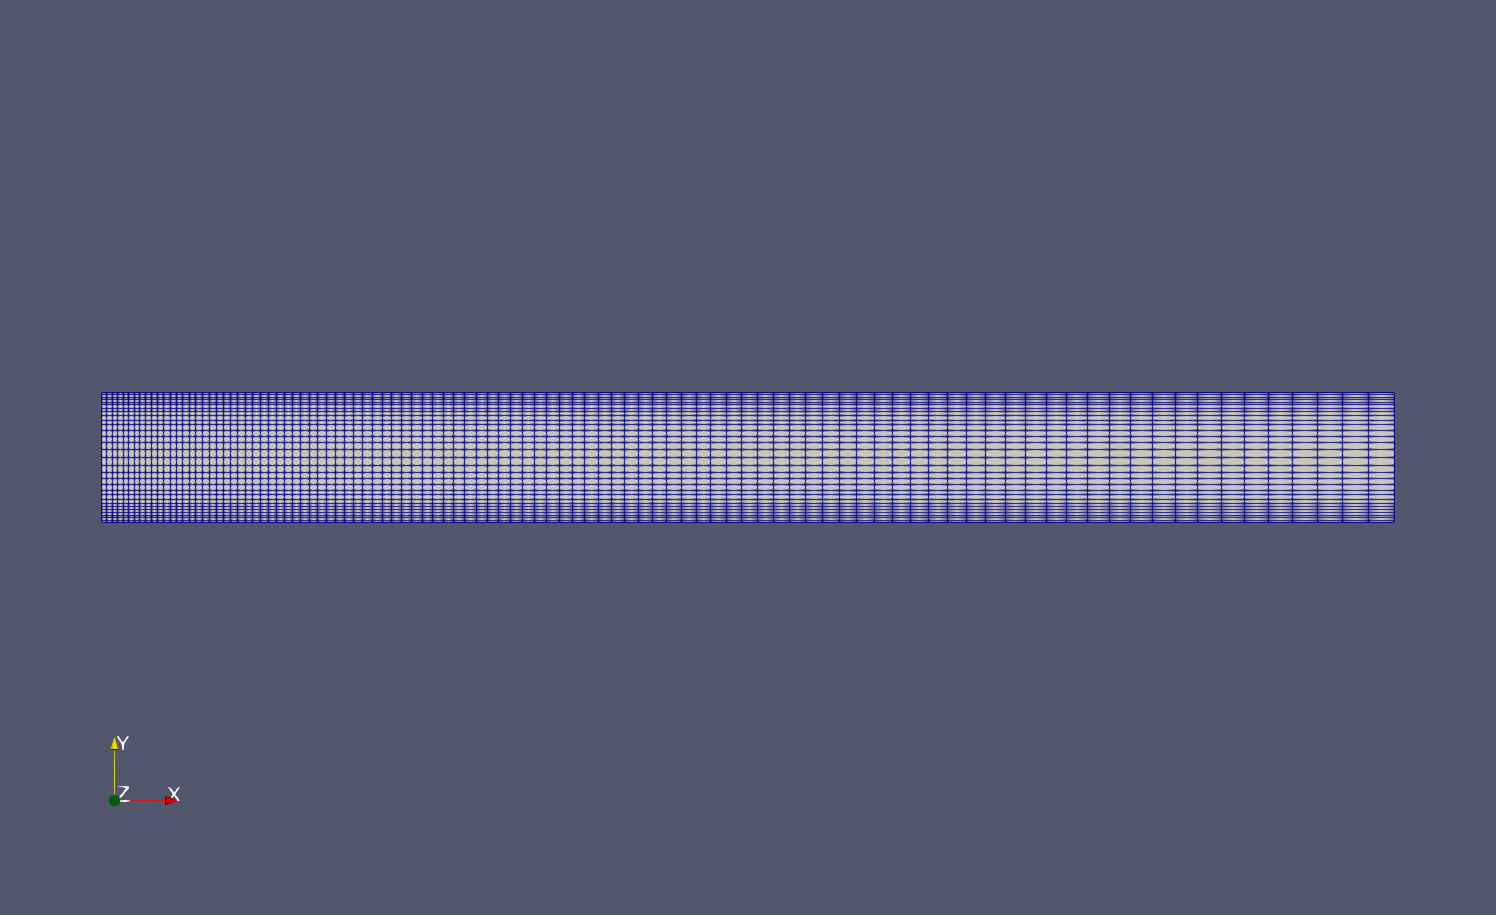
\includegraphics[width=0.8\textwidth,trim={0cm 12cm 0 12cm},clip]{2D_mesh.png}
			\caption{Mesh}
		\end{subfigure}
 		\begin{subfigure}{\textwidth}
 			\centering
 			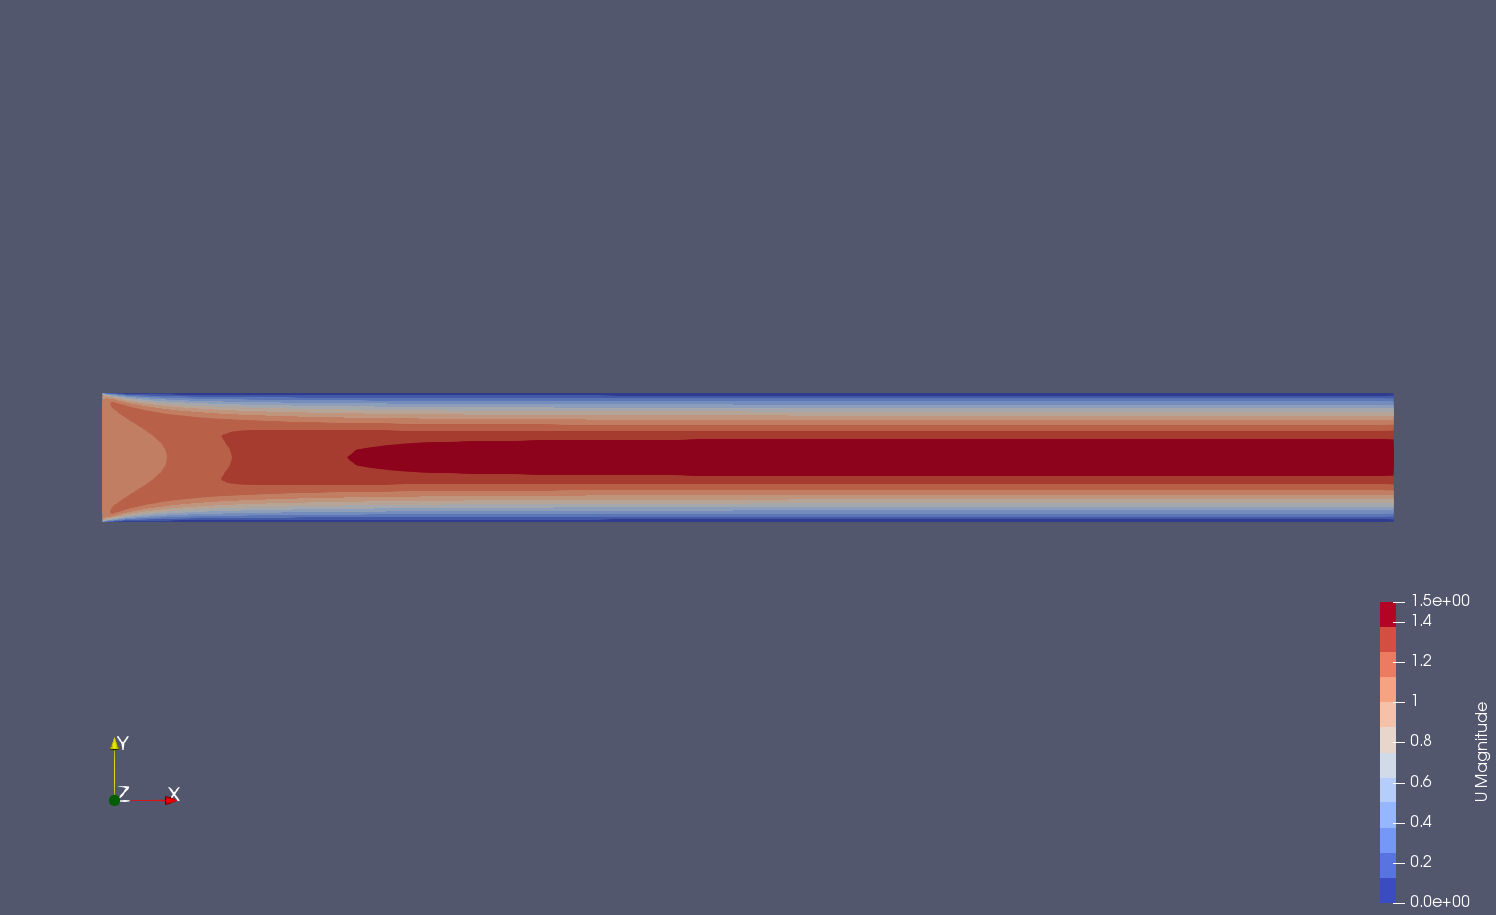
\includegraphics[width=0.8\textwidth,trim={0cm 12cm 0 12cm},clip]{2D_velocity.png}
 			\caption{Velocity}
 		\end{subfigure}	
 	\end{figure}
 	
	\newpage
 	\item Extend the previous case, into a 3D square pipe.
 	
	\begin{figure}[h]
		\centering
 		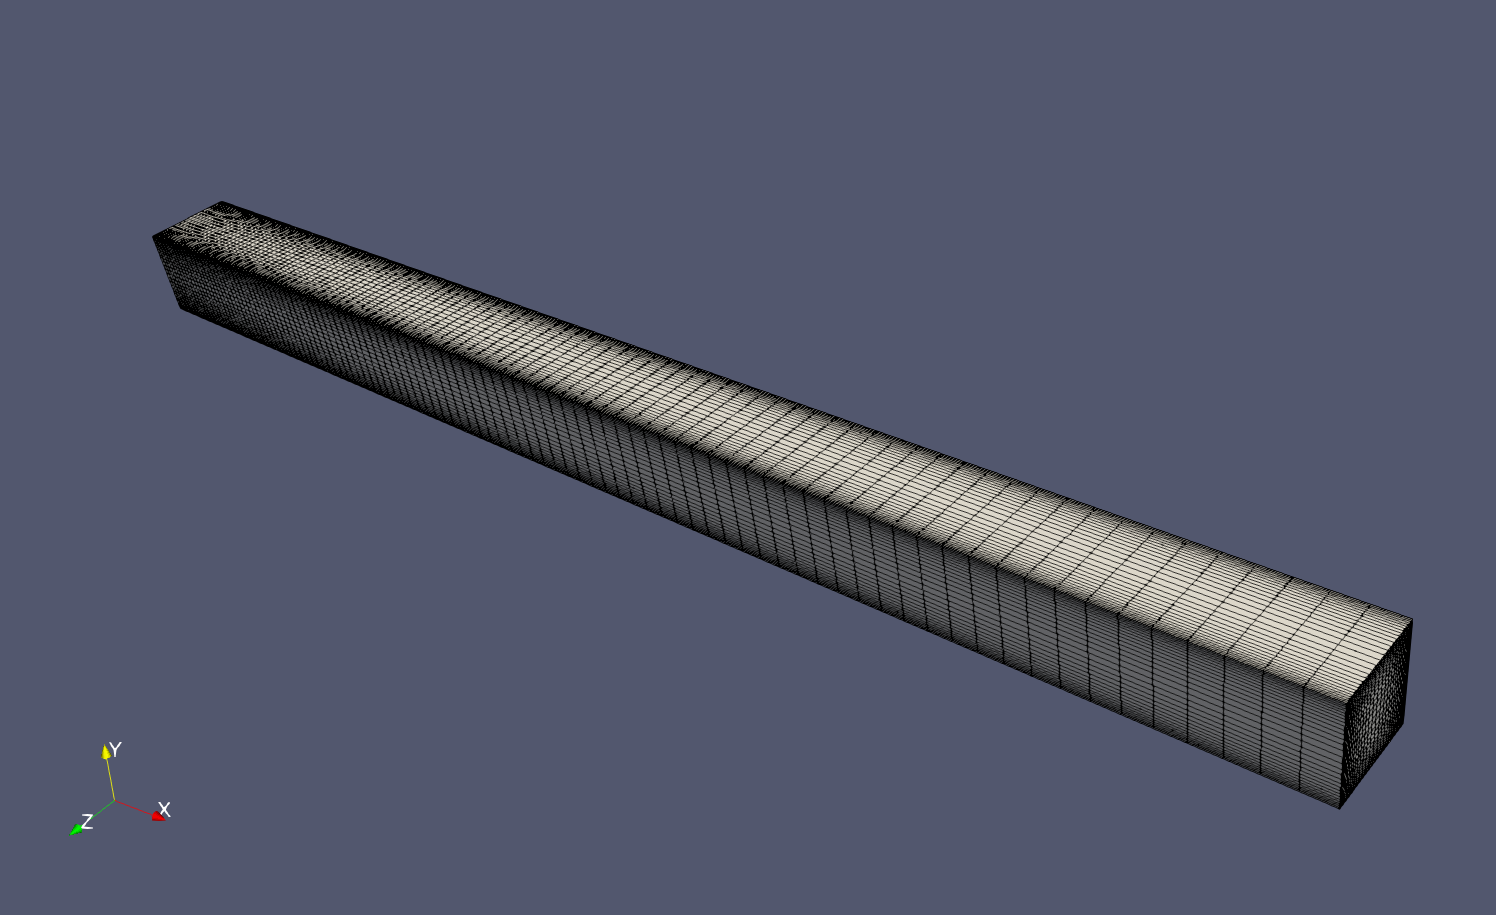
\includegraphics[width=0.8\textwidth]{3D_mesh2.png}
 		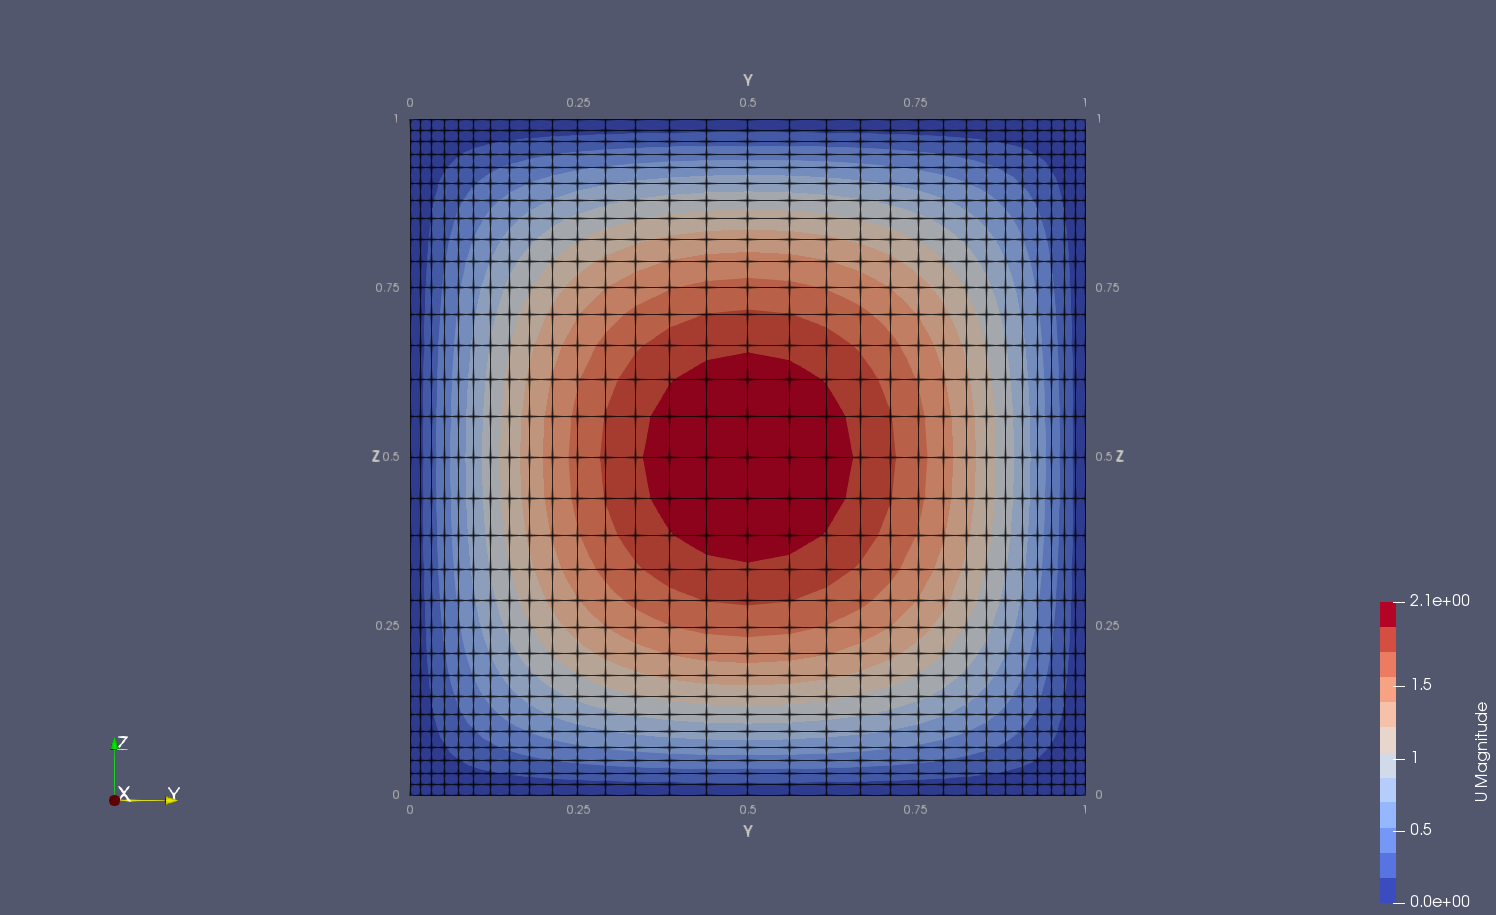
\includegraphics[width=0.8\textwidth]{3D_velocity.png}
	\end{figure}

	
\end{enumerate}
	
%\section*{Πρώτα βήματα στο \en{OpenFOAM}}
%\begin{enumerate}
%	\item Εγκαταστήστε ένα λειτουργικό σύστημα \en{Linux} στον υπολογιστή σας (κατά προτίμηση την τελευταία έκδοση των \en{\href{https://ubuntu.com/}{Ubuntu}}), είτε σαν \en{dual-boot} είτε με την βοήθεια ενός \en{Virtual Machine}. Στην συνέχεια εξοικειωθείτε με την χρήση του \en{terminal} των \en{Linux} [\href{https://ubuntu.com/tutorials/command-line-for-beginners#6-a-bit-of-plumbing}{1}, \href{https://www.howtogeek.com/140679/beginner-geek-how-to-start-using-the-linux-terminal/}{2}] και του λειτουργικού συστήματος γενικότερα.
%	
%	\item Εγκαταστήστε με επιτυχία την τελευταία έκδοση του λογισμικού \en{OpenFOAM} και του \en{post-process} εργαλείου \en{ParaView} από την \href{https://openfoam.org/}{επίσημη ιστοσελίδα}, σύμφωνα με τις οδηγίες που παρέχονται.
%	
%	\item Με την βοήθεια του \en{User Guide} που παρέχεται από την ιστοσελίδα του \en{OpenFOAM} τρέχτε το \en{case} με όνομα \en{cavity}, χρησιμοποιώντας τον ασυμπίεστο λύτη (\en{solver}) \en{\tt icoFoam}. Για να το κάνετε αυτό αντιγράψτε τον φάκελο με το αντίστοιχο \en{tutorial case} στον προσωπικό σας φάκελο που δημιουργήσατε κατά την εγκατάσταση του \en{OpenFOAM} στο \en{{\tt \$HOME} directory} σας, είτε χειροκίνητα από τον φάκελο που βρίσκεται στην διαδρομή (π.χ. για την έκδοση \en{OpenFOAM v8}):
%	
%	{\tt \tab \en{/opt/openfoam8/tutorials/incompressible/icoFoam/cavity/cavity} }
%	
%	 είτε με την εντολή
%	
%	\en{\tt \tab \$ cp -r \$FOAM\_TUTORIALS/incompressible/icoFoam/cavity/cavity \$FOAM\_RUN}
%	
%	Για να επιλύσετε το συγκεκριμένο \en{tutorial}, τρέξτε τις παρακάτω εντολές:
%	
%	\en{\tt %
%	\tab \$ cd FOAM\_RUN/cavity	\\%
%	\tab \$ blockMesh \\%
%	\tab \$ icoFoam \\%
%	\tab \$ paraFoam
% 	}
% 
%	Στον φάκελο που μόλις δημιουργήσατε μπορείτε να εξοικειωθείτε με την γεωμετρία του προβλήματος, τις παραμέτρους (\en{\tt constant/transportProperties}), συνοριακές συνθήκες, χρονικά βήματα $\Delta t$, χρόνους εγγραφής αποτελεσμάτων. Επίσης εξοικειωθείτε με την βοήθεια του \en{User Guide} με το \en{post-process} εργαλείο \en{ParaView} και τις επιλογές του.
%	
%	\item Διαμορφώστε κατάλληλα το \en{cavity case} που μόλις δημιουργήσατε, έτσι ώστε να προσομοιώσετε την 2\en{D} ροή ανάμεσα σε παράλληλες πλάκες. Υπενθυμίζεται πως το προφίλ εξόδου πρέπει να είναι παραβολικής μορφής και η μέγιστη ταχύτητα εξόδου ίση με τα $3/2$ της ομοιόμορφης ταχύτητας εισόδου.
%	
%	Οι συνοριακές συνθήκες για την ταχύτητα πρέπει να είναι \en{\tt noSlip} στα τοιχώματα (\en{walls}), \en{\tt uniform} στην είσοδο (\en{inlet}), ενώ \en{\tt zeroGradient} στην έξοδο (\en{outlet}) του αγωγού. Αντίστοιχα, η πίεση πρέπει να είναι παντού \en{\tt zeroGradient}, εκτός από την έξοδο του αγωγού όπου είναι μηδενική (το ρευστό θεωρείται πως εξέρχεται στην ατμόσφαιρα άρα η σχετική πίεση του αγωγού σε εκείνο το σημείο είναι μηδέν). 
%	
%	\item Δημιουργείστε έναν καινούριο \en{solver} με τον όνομα \en{\tt laplaceFoam} που να λύνει την εξίσωση \en{Laplace} σε μια ορθογωνική πλάκα, με συνοριακές και αρχικές συνθήκες όπως φαίνονται στην παρακάτω εικόνα. 
%	
%	Χρησιμοποιείστε $T_w=10~K,~L=2~m$ και $H=1~m$.
%	
%	\begin{center}
%		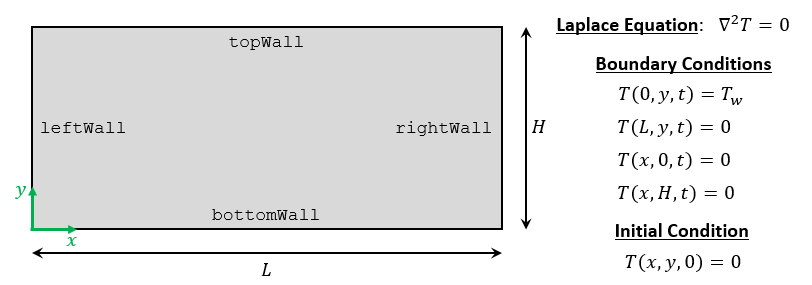
\includegraphics[scale = 0.45]{laplace.jpg}
%	\end{center}
%	
%	Για την δημιουργία του καινούριου \en{solver}, αντιγράψτε έναν ήδη υπάρχον από τον φάκελο \en{\tt \$FOAM\_SOLVERS} σε έναν νέο φάκελο με όνομα \en{\tt applications} στο \en{local directory} (π.χ. \en{\tt \$HOME/OpenFoam/<USER>-8/}, όπου \en{\tt <USER>} το όνομα του χρήστη). Για ευκολία, να χρησιμοποιηθεί ο \en{solver} \en{\tt electrostaticFoam} που βρίσκεται στην κατηγορία λυτών \en{electromagnetics}.
%	
%	Μετονομάστε τον φάκελο που περιέχει τον καινούριο λύτη από \en{\tt electrostaticFoam} σε \en{\tt laplaceFoam}, το αρχείο \en{\tt electrostaticFoam.c} σε \en{\tt laplaceFoam.c} και τροποποιείστε τα περιεχόμενά του αρχείου \en{\tt ./Make/files} έτσι ώστε να γράφει:
%	
%%	\hspace{0.4cm}
%%	\begin{minipage}{0.6\textwidth}
%%	\begin{myframe}
%%	\en{\tt %
%%	 {\small 1} ~laplaceFoam.C \\%
%%	 {\small 2} ~\\%	
%%	 {\small 3} ~EXE = \$(FOAM\_USER\_APPBIN)/laplaceFoam}
%% 	\end{myframe}
%%	\end{minipage}
%
%	\hspace{0.4cm}
%	\begin{minipage}{0.92\textwidth}
%	\begin{myframe}
%		\en{\tt %
%			laplaceFoam.C \\%
%			\\%	
%			EXE = \$(FOAM\_USER\_APPBIN)/laplaceFoam}
%	\end{myframe}
%	\end{minipage}
%
%	Τροποιείστε κατάλληλα τα περιεχόμενα των αρχείων \en{\tt laplaceFoam.c} και \en{\tt createFields.h} έτσι ώστε να λύνεται η μόνο εξίσωση \en{Laplace} για το \en{\tt scalarField} με όνομα \en{\tt T}. 
%	
%	Για να κάνετε \en{compile} τον λύτη, τρέξτε στον φάκελο την εντολή
%	
%	\en{\tt \tab \$ wmake}
%	
%	Σε περίπτωση που χρειαστεί να διαγράψετε το \en{executable} αρχείο που υπάρχει ήδη, χρησιμοποιείστε την εντολή
%	
%	\en{\tt \tab \$ wclean}
%	
%	Τέλος τρέξτε το \en{case} και ελέγξτε τα αποτελέσματά σας.
%	
%	\item Σε αυτό το βήμα θα μοντελοποιηθεί η μετάδοση θερμότητας σε δυο εφαπτομενικά  χωρία, το ένα θα είναι μία στερεή πλάκα, όπου θα λυθεί η εξίσωση \en{Laplace} και το άλλο ο αέρας, όπου θα λυθεί η εξίσωση \en{Poisson}. Στο παρακάτω σχήμα φαίνονται ακριβώς τα χαρακτηριστικά, οι εξισώσεις και οι συνοριακές συνθήκες που θα χρησιμοποιηθούν. Μπορεί να χρησιμοποιηθεί ο λύτης \en{\tt laplaceFoam} που ήδη έχετε κατασκευάσει στο προηγούμενο βήμα, και να τροποποιηθεί για το συγκεκριμένο πρόβλημα.
%	
%	\begin{center}
%		\includegraphics[scale = 0.5]{regions.jpg}
%	\end{center}
%	
%	Για να επιτευχθεί αυτό, θα πρέπει να δημιουργηθεί ένα \en{block} στο μέγεθος και των δύο χωρίων από το \en{\tt blockMeshDict}, και μετά χρησιμοποιώντας το εργαλείο \en{\tt topoSet} του \en{OpenFOAM} να χωριστούν σε δύο \en{regions}. Το ένα \en{region} να ονομαστεί \en{solid} και το άλλο \en{air}. Στην διεπιφάνεια των δύο \en{regions} θα πρέπει να οριστούν κατάλληλες οριακές συνθήκες για την σωστή λύση των εξισώσεων. Πιο συγκεκριμένα, θα πρέπει η τιμή της θερμοκρασίας και η παράγωγός της στο \en{interface} των δύο περιοχών να είναι ίσες
%	
%	$$ T_{air} = T_{solid} $$
%	
%	$$ k_{air} \dfrac{\partial T}{\partial n} \Bigg|_{air} = k_{solid} \dfrac{\partial T}{\partial n} \Bigg|_{solid} $$
%	
%	όπου $k$ είναι ο συντελεστής θερμικής αγωγιμότητας του κάθε χωρίου.
%	
%	Η οριακή συνθήκη που χρησιμοποιείται είναι η:
%	
%	\tab \en{\tt compressible::turbulentTemperatureCoupledBaffleMixed}
%
%	και μπορεί να βρεθεί ο τρόπος χρήσης της, όπως και ο τρόπος δημιουργίας \en{regions} με το \en{\tt topoSet} (αρχείο \en{\tt topoSetDict}), από τα \en{tutorial cases} του λύτη \en{\tt chtMultiRegionFoam}, που βρίσκεται στην κατηγορία \en{heat transfer}. 
%	
%	Επιπλέον, θα πρέπει να δημιουργηθούν στον \en{solver} δύο διαφορετικά πλέγματα, όπου στο ένα (\en{meshA}) θα λυθεί η εξίσωση \en{Poisson} για τον αέρα και στο άλλο (\en{meshS}) θα λυθεί η εξίσωση \en{Laplace} στο στερεό. Αυτό συνεπάγεται, πως θα υπάρχουν δύο διαφορετικές μεταβλητές (\en{\tt scalarFields}) στο αρχείο \en{\tt createFields.h}, μία για την θερμοκρασία στον αέρα \en{\tt Tair} και μία για την θερμοκρασία στο στερεό \en{\tt Tsolid}. Αντίστοιχα, όπως αναφέρθηκε προηγουμένως, θα πρέπει να υπάρχουν δύο διαφορετικές εξισώσεις στο αρχείο \en{\tt laplaceFoam.c}, η \en{Poisson} για την \en{\tt Tair} στο \en{meshA}, και η \en{Laplace} για την \en{\tt Tsolid} στο \en{meshS}.
%	
%	Θα πρέπει να υπάρχουν, αντίστοιχα και στο \en{case} δύο διαφορετικά αρχεία για τις συνοριακές συνθήκες και να τοποθετηθούν στους φακέλους που θα δημιουργηθούν μετά την χρήση του \en{\tt topoSet}, στις διαδρομές \en{\tt ./0/air} και \en{\tt ./0/solid} . Σε κάθε αρχείο συνοριακής συνθήκης θα πρέπει να προστεθεί και η συνθήκη για την διεπιφάνεια. Ο ακριβής τίτλος του συνόρου των διεπιφανειών (μία για κάθε \en{region}) δημιουργείται αυτόματα από την εντολή \en{\tt topoSet} και μπορεί να βρεθεί στις διαδρομές \en{\tt ./constant/air} και \en{\tt ./constant/solid}. Τέλος, πρέπει να σημειωθεί, πως για την σωστή λειτουργία της συνοριακής συνθήκης \en{\tt BaffleMixed} θα πρέπει να δημιουργηθούν δυο \en{scalar} μεταβλητές π.χ. \en{kappaA} και \en{kappaS} οι οποίες θα έχουν την τιμή των σταθερών $k_{air}$ και $k_{solid}$ σε ολόκληρο το \en{region} που αντιστοιχεί σε κάθε μεταβλητή.
%	
%	Παράδειγμα της συνοριακής συνθήκης για την μεταβλητή \en{\tt Tair} φαίνεται παρακάτω.
%	
%	\hspace{0.4cm}
%	\begin{minipage}{0.92\textwidth}
%	\begin{myframe}
%	\en{\tt %
%    air\_to\_solid\\%
%		\{\\%
%		\tab	type  ~~~~~~~~~~          compressible::turbulentTemperatureCoupledBaffleMixed;\\%
%		\tab	value  ~~~~~~~~~         \$internalField;\\%
%		\tab	Tnbr   ~~~~~~~~~~         Tsolid;\\%
%		\tab	kappaMethod ~~~    lookup;\\%
%		\tab	kappa    ~~~~~~~~~       kappaA;\\%
%		\}\\%
%	}
%	\end{myframe}
%	\end{minipage}
%	
%	
%	
%	
%	
%	
%	
%
%	
%	
%\end{enumerate}










\end{document}